\chapter{Experimental Analysis of CNN Frequency Sensitivity}

\section{Chapter Objective and Scope}
\label{sec:objectif_positionnement_chapitre4}

In the previous chapter, we showed that Fourier functions play a special role
in the analysis of convolution operators. In the idealized linear setting, certain
frequency directions emerge as preferred directions of the convolutional operator. In a
real CNN, which includes ReLU and max-pooling, this property is no longer global or exact,
but it can still be interpreted locally through the model's Jacobian.

The objective of this chapter is therefore to test experimentally whether this frequency sensitivity remains
observable in a CNN trained on real data. We do not aim to reproduce all
the experiments of Tsuzuku and Sato~\cite{tsuzuku2019structural}, but to adopt their central
mechanism: systematically testing perturbations constructed from Fourier frequencies and
measuring their ability to change the model's predictions.

Our protocol focuses on \texttt{VGGSmallBN}, a VGG-style architecture with batch normalization,
trained on CIFAR-10 and CIFAR-100. For each frequency $(u,v)$,
we construct a universal Fourier perturbation and then measure the proportion of
predictions that change. This measure, called the \textit{fool ratio}, allows us to construct a
frequency sensitivity map of the model.

Our reproduction is deliberately more limited than that of Tsuzuku and Sato, but retains the essential elements: constructing a Fourier perturbation,
controlling its amplitude, calculating the \textit{fool ratio}, and generating a frequency heatmap.

The main amplitude is set to
\[
    \epsilon = 10/255,
\]
as in the CIFAR experiments in the original paper. We then add two experimental
controls: a comparison with random noise of the same amplitude and a sweep over
several values of $\epsilon$.

Finally, unlike the paper's heatmap algorithm, which evaluates each frequency on a
minibatch, we evaluate each frequency on the full test set. This makes the computation
more expensive but provides a more stable estimate of the \textit{fool ratio}.

\section{Experimental Setup}

\subsection{Datasets}

We use CIFAR-10 and CIFAR-100. Both datasets contain RGB images of
size $32\times32$, allowing us to retain the same frequency domain in both experiments:
\[
    (u,v) \in \{0,\dots,31\}^2.
\]

CIFAR-10 contains $10$ classes and provides a relatively stable initial setting for reproduction.
CIFAR-100 contains $100$ classes at the same image resolution; the task is therefore more difficult,
since the categories are more numerous and often visually similar. Comparing the
two allows us to observe whether frequency sensitivity persists as classification becomes more fine-grained.

\subsection{Architecture}

For this experimental reproduction, we use a VGG-style convolutional architecture
with batch normalization, which we call \texttt{VGGSmallBN}. The aim is not to reproduce
a historical VGG architecture exactly~\cite{simonyan2015very}, but to retain its general
principle: stacking several simple convolutional blocks consisting of $3\times3$ convolutions,
batch normalization, ReLU activations, and spatial reduction layers.

The network consists of four convolutional blocks. Each block contains two
$3\times3$ convolutions, each followed by batch normalization and a ReLU activation. The block ends
with \textit{max-pooling} of size $2\times2$, which halves the spatial resolution. The
classification head then applies \textit{adaptive average pooling}, flattens the resulting tensor, and
uses a final linear layer. This architecture is summarized in Figure~\ref{fig:vgg_small_bn_v3}.

\begin{figure}[H]
    \centering
    \resizebox{\textwidth}{!}{
    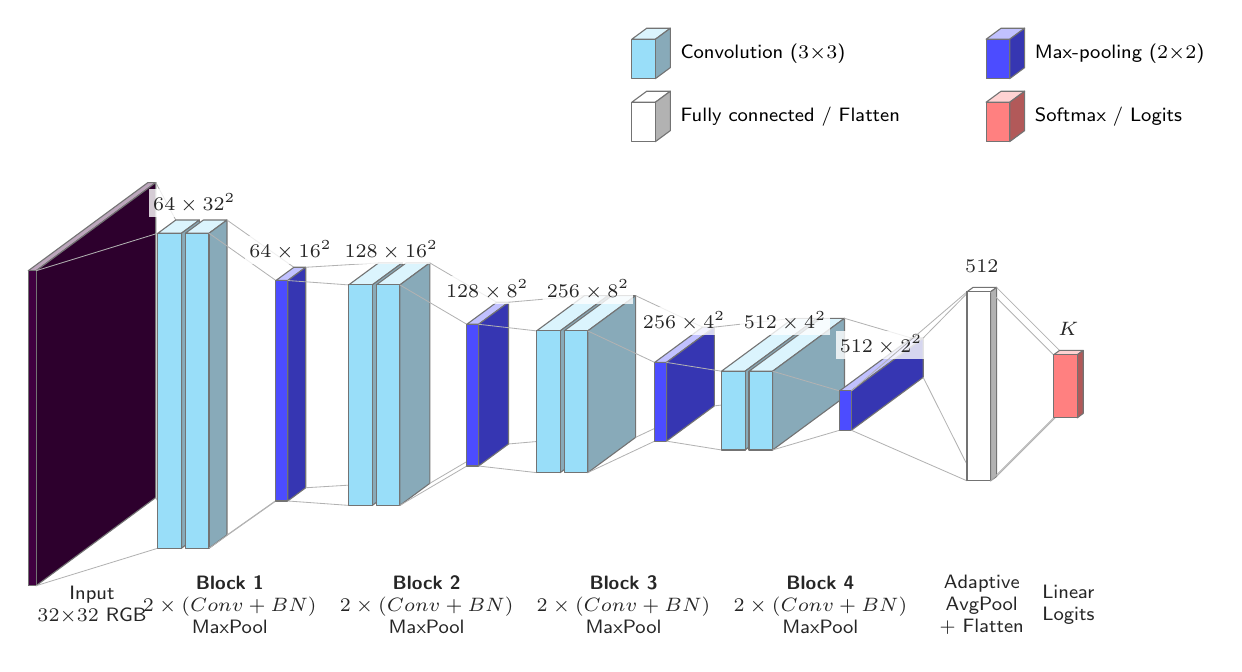
\begin{tikzpicture}[
        x={(1cm,0cm)},
        y={(0cm,1cm)},
        z={(0.38cm,0.28cm)},
        font=\sffamily\footnotesize,
        dimlabel/.style={
            align=center,
            text=black!85,
            font=\sffamily\scriptsize,
            fill=white,
            fill opacity=0.8,
            text opacity=1,
            inner sep=1.5pt
        },
        blocklabel/.style={
            align=center,
            text=black!85,
            font=\sffamily\scriptsize
        }
    ]

    % --- Définition des couleurs ---
    \colorlet{colIn}{violet!50!black}
    \colorlet{colConv}{cyan!40}
    \colorlet{colPool}{blue!70}
    \colorlet{colFC}{white}
    \colorlet{colSoftmax}{red!50}

    % --- Macros de dessin ---
    \def\drawbox#1#2#3#4#5{
        \pgfmathsetmacro{\yy}{-#2/2}
        \pgfmathsetmacro{\zz}{-#3/2}
        \filldraw[fill=#5!35!white, draw=black!55, line width=0.4pt, line join=round]
            (#1,\yy+#2,\zz) -- (#1+#4,\yy+#2,\zz) -- (#1+#4,\yy+#2,\zz+#3) -- (#1,\yy+#2,\zz+#3) -- cycle;
        \filldraw[fill=#5!70!black, draw=black!55, line width=0.4pt, line join=round]
            (#1+#4,\yy,\zz) -- (#1+#4,\yy,\zz+#3) -- (#1+#4,\yy+#2,\zz+#3) -- (#1+#4,\yy+#2,\zz) -- cycle;
        \filldraw[fill=#5, draw=black!55, line width=0.4pt, line join=round]
            (#1,\yy,\zz) -- (#1+#4,\yy,\zz) -- (#1+#4,\yy+#2,\zz) -- (#1,\yy+#2,\zz) -- cycle;
    }

    \def\connect#1#2#3#4#5#6{
        \draw[black!30, line width=0.3pt, line join=round] (#1, #2/2, -#3/2) -- (#4, #5/2, -#6/2);
        \draw[black!30, line width=0.3pt, line join=round] (#1, -#2/2, -#3/2) -- (#4, -#5/2, -#6/2);
        \draw[black!30, line width=0.3pt, line join=round] (#1, #2/2, #3/2) -- (#4, #5/2, #6/2);
        \draw[black!30, line width=0.3pt, line join=round] (#1, -#2/2, #3/2) -- (#4, -#5/2, #6/2);
    }

    % ==================================================================
    % ARCHITECTURE DU RESEAU
    % ==================================================================

    % --- Entrée (Rendu comme une image carrée 32x32) ---
    \drawbox{0.0}{4.0}{4.0}{0.1}{colIn} % Hauteur 4, Profondeur 4 = Carré
    \node[blocklabel] at (0.05, -2.8, 0) {Input\\$32{\times}32$ RGB};
    \connect{0.1}{4.0}{4.0}{1.0}{4.0}{0.6}

    % --- Bloc 1 (avec micro-espace entre Conv) ---
    \drawbox{1.0}{4.0}{0.6}{0.3}{colConv} % Conv 1
    \drawbox{1.35}{4.0}{0.6}{0.3}{colConv} % Conv 2 (Ecart de 0.05)
    \node[dimlabel] at (1.35, 2.3, 0) {$64 \times 32^2$};
    
    \connect{1.65}{4.0}{0.6}{2.5}{2.8}{0.6}
    \drawbox{2.5}{2.8}{0.6}{0.15}{colPool}
    \node[dimlabel] at (2.57, 1.7, 0) {$64 \times 16^2$};
    
    \node[blocklabel] at (1.8, -2.8, 0) {\textbf{Block 1}\\$2\times(\text{Conv}+\text{BN})$\\MaxPool};
    \connect{2.65}{2.8}{0.6}{3.5}{2.8}{1.0}

    % --- Bloc 2 ---
    \drawbox{3.5}{2.8}{1.0}{0.3}{colConv}
    \drawbox{3.85}{2.8}{1.0}{0.3}{colConv}
    \node[dimlabel] at (3.85, 1.7, 0) {$128 \times 16^2$};

    \connect{4.15}{2.8}{1.0}{5.0}{1.8}{1.0}
    \drawbox{5.0}{1.8}{1.0}{0.15}{colPool}
    \node[dimlabel] at (5.07, 1.2, 0) {$128 \times 8^2$};

    \node[blocklabel] at (4.3, -2.8, 0) {\textbf{Block 2}\\$2\times(\text{Conv}+\text{BN})$\\MaxPool};
    \connect{5.15}{1.8}{1.0}{6.0}{1.8}{1.6}

    % --- Bloc 3 ---
    \drawbox{6.0}{1.8}{1.6}{0.3}{colConv}
    \drawbox{6.35}{1.8}{1.6}{0.3}{colConv}
    \node[dimlabel] at (6.35, 1.2, 0) {$256 \times 8^2$};

    \connect{6.65}{1.8}{1.6}{7.5}{1.0}{1.6}
    \drawbox{7.5}{1.0}{1.6}{0.15}{colPool}
    \node[dimlabel] at (7.57, 0.8, 0) {$256 \times 4^2$};

    \node[blocklabel] at (6.8, -2.8, 0) {\textbf{Block 3}\\$2\times(\text{Conv}+\text{BN})$\\MaxPool};
    \connect{7.65}{1.0}{1.6}{8.5}{1.0}{2.4}

    % --- Bloc 4 ---
    \drawbox{8.5}{1.0}{2.4}{0.3}{colConv}
    \drawbox{8.85}{1.0}{2.4}{0.3}{colConv}
    \node[dimlabel] at (8.85, 0.8, 0) {$512 \times 4^2$};

    \connect{9.15}{1.0}{2.4}{10.0}{0.5}{2.4}
    \drawbox{10.0}{0.5}{2.4}{0.15}{colPool}
    \node[dimlabel] at (10.07, 0.5, 0) {$512 \times 2^2$};

    \node[blocklabel] at (9.3, -2.8, 0) {\textbf{Block 4}\\$2\times(\text{Conv}+\text{BN})$\\MaxPool};
    \connect{10.15}{0.5}{2.4}{11.2}{2.4}{0.2}

    % --- Tête finale ---
    \drawbox{11.2}{2.4}{0.2}{0.3}{colFC}
    \node[dimlabel] at (11.35, 1.5, 0) {$512$};
    \node[blocklabel] at (11.35, -2.8, 0) {Adaptive\\AvgPool\\+ Flatten};
    \connect{11.5}{2.4}{0.2}{12.3}{0.8}{0.2}

    \drawbox{12.3}{0.8}{0.2}{0.3}{colSoftmax}
    \node[dimlabel] at (12.45, 0.7, 0) {$K$};
    \node[blocklabel] at (12.45, -2.8, 0) {Linear\\Logits};

    % --- Légende ---
    \begin{scope}[shift={(7.0, 4.2)}] 
        \begin{scope}[shift={(0, 0)}]
            \drawbox{0}{0.5}{0.5}{0.3}{colConv}
            \node[right, font=\sffamily\scriptsize] at (0.4, 0, 0) {Convolution ($3{\times}3$)};
        \end{scope}
        \begin{scope}[shift={(0, -0.8)}]
            \drawbox{0}{0.5}{0.5}{0.3}{colFC}
            \node[right, font=\sffamily\scriptsize] at (0.4, 0, 0) {Fully connected / Flatten};
        \end{scope}
        \begin{scope}[shift={(4.5, 0)}]
            \drawbox{0}{0.5}{0.5}{0.3}{colPool}
            \node[right, font=\sffamily\scriptsize] at (0.4, 0, 0) {Max-pooling ($2{\times}2$)};
        \end{scope}
        \begin{scope}[shift={(4.5, -0.8)}]
            \drawbox{0}{0.5}{0.5}{0.3}{colSoftmax}
            \node[right, font=\sffamily\scriptsize] at (0.4, 0, 0) {Softmax / Logits};
        \end{scope}
    \end{scope}

    \end{tikzpicture}
    }
    \caption{Illustration of the \texttt{VGGSmallBN} architecture used, where $K$ denotes the number of classes in the dataset: $K=10$ for CIFAR-10 and $K=100$ for CIFAR-100.}
    \label{fig:vgg_small_bn_v3}
\end{figure}

\subsection{Training Parameters}

\begin{table}[H]
    \centering
    \small
    \begin{tabular}{|l|l|}
        \hline
        \textbf{Parameter} & \textbf{Selected value} \\
        \hline
        Number of epochs & $100$ \\
        \hline
        Optimizer & SGD \\
        \hline
        Initial learning rate & $0.1$ \\
        \hline
        Momentum & $0.9$ \\
        \hline
        Weight decay & $5\cdot 10^{-4}$ \\
        \hline
        Scheduler & Cosine annealing \\
        \hline
        Batch size & $256$ \\
        \hline
        Datasets & CIFAR-10 and CIFAR-100 \\
        \hline
        Architecture & \texttt{VGGSmallBN} \\
        \hline
    \end{tabular}
    \caption{Training parameters used for the \texttt{VGGSmallBN} models.}
    \label{tab:parametres_entrainement_vgg}
\end{table}

Momentum stabilizes weight updates and
accelerates optimization. \textit{Weight decay} acts as a regularizer: it penalizes
excessively large weights, thereby limiting the risk of overfitting.

The initial learning rate is set to $0.1$ and then gradually reduced using a
\textit{cosine annealing} scheduler. The idea is to let the model learn quickly at the beginning of
training and then make finer adjustments toward the end. Finally,
we train the model for $100$ epochs with a batch size of $256$, allowing
efficient use of the available GPU while maintaining stable training.

\subsection{Baseline Performance}

\begin{table}[H]
    \centering
    \small
    \begin{tabular}{|l|c|c|c|}
        \hline
        \textbf{Dataset} & \textbf{Number of classes} & \textbf{Validation} & \textbf{Test} \\
        \hline
        CIFAR-10 & $10$ & $93.86\,\%$ & $93.07\,\%$ \\
        \hline
        CIFAR-100 & $100$ & $73.04\,\%$ & $72.55\,\%$ \\
        \hline
    \end{tabular}
    \caption{Baseline performance of the \texttt{VGGSmallBN} models before perturbations are added.}
    \label{tab:performance_reference_vgg}
\end{table}

The difference between the two datasets is expected: CIFAR-100 contains ten times as many classes as
CIFAR-10, with categories that are often more visually similar. In both cases, performance
is high enough for the perturbation study to be interpretable: the models are
not perfect, but they serve as credible baseline classifiers.

\section{Constructing Fourier Perturbations}
\label{sec:construction_perturbations_fourier}

The general idea is to construct a universal perturbation. Unlike a conventional adversarial attack,
the perturbation is not optimized separately for each image.
It depends only on a frequency $(u,v)$ and an amplitude $\epsilon$.
We then examine whether this frequency direction, although it is not a global eigenvector
of the real network, is sufficient to change the model's predictions on a large number of images.

\subsection{Single Fourier Attack}
\label{subsec:single_fourier_attack}

The \textit{Single Fourier Attack} (SFA) proposed by Tsuzuku and Sato~\cite{tsuzuku2019structural}
constructs a perturbation from a single Fourier frequency. The main idea
is simple: instead of optimizing a different perturbation for each image, we choose a
frequency $(u,v)$, construct the corresponding spatial pattern, and then add that same pattern to all
images.

In our protocol, a frequency is represented by a pair
\[
    (u,v) \in \{0,\dots,N-1\}^2,
\]
where $N$ denotes the spatial size of the image.

For a given frequency $(u,v)$, let $\delta_{u,v}$ denote the perturbation constructed from that
frequency. The perturbed image is then defined by
\begin{equation}
    \tilde{x}_{i}
    =
    \operatorname{clip}_{[0,1]}\left(x_i + \delta_{u,v,i}\right)
    =
    \begin{cases}
        0, & \text{if } x_i + \delta_{u,v,i} < 0, \\
        x_i + \delta_{u,v,i}, & \text{if } x_i + \delta_{u,v,i} \in [0,1], \\
        1, & \text{if } x_i + \delta_{u,v,i} > 1.
    \end{cases}
    \label{eq:single_fourier_attack}
\end{equation}
Here, $x$ is the original image, $\tilde{x}$ is the perturbed image, and clipping ensures that
pixel values remain within the valid interval $[0,1]$.

In practice, for each frequency $(u,v)$, we first construct a real-valued spatial pattern
$p_{u,v}$. This pattern is then normalized in the $\ell_\infty$ norm so that its maximum amplitude
equals the chosen amplitude $\epsilon$:
\begin{equation}
    \delta_{u,v}
    =
    \epsilon
    \frac{p_{u,v}}{\|p_{u,v}\|_\infty}.
    \label{eq:normalisation_sfa}
\end{equation}

Thus, if one frequency achieves a higher \textit{fool ratio} than another,
this is not because it was tested with a larger perturbation, but because its
frequency direction disrupts the model more.

For the RGB images in CIFAR-10 and CIFAR-100, the same spatial pattern is applied to all three color
channels.
The final perturbation therefore has the same frequency structure in each channel. After the perturbation
is added, the image is clipped to the interval $[0,1]$ and normalized using the statistics of the dataset
before being passed to the model.

Algorithm~\ref{algo:single_fourier_attack} summarizes the procedure used in our implementation.

\begin{algorithm}[H]
\caption{Single Fourier Attack used in our protocol}
\label{algo:single_fourier_attack}
\begin{algorithmic}
\State \textbf{input}: image $x$, frequency $(u,v)$, amplitude $\epsilon$
\State \textbf{output}: perturbed image $\tilde{x}$
\State
\State Construct the real-valued spatial pattern $p_{u,v}$
\State Normalize this pattern in the $\ell_\infty$ norm:
\State \hspace{0.5cm} $\delta_{u,v} \leftarrow \epsilon \dfrac{p_{u,v}}{\|p_{u,v}\|_\infty}$
\State Add the perturbation to the image:
\State \hspace{0.5cm} $x_{\mathrm{pert}} \leftarrow x + \delta_{u,v}$
\State Apply clipping:
\State \hspace{0.5cm} $\tilde{x} \leftarrow \operatorname{clip}_{[0,1]}(x_{\mathrm{pert}})$
\State \Return $\tilde{x}$
\end{algorithmic}
\end{algorithm}

\subsection{Amplitude Control}

In our main protocol, we use the same bound as in the original paper
for CIFAR:
\[
    \epsilon = \frac{10}{255}.
\]
This value means that each pixel can be changed by at most $10$ levels on a scale from
$0$ to $255$.

For each frequency $(u,v)$, the perturbation is normalized to satisfy
\[
    \|\delta_{u,v}\|_{\infty} \leq \epsilon.
\]

After the perturbation is added, the image is clipped to the valid interval $[0,1]$, as
in Equation~\eqref{eq:single_fourier_attack}.

As an example, Figure~\ref{fig:sfa_spatial_pattern_vgg_cifar10} shows the spatial pattern obtained
for frequency $(16,24)$, which corresponds to the best direction found on CIFAR-10.

\begin{figure}[H]
    \centering
    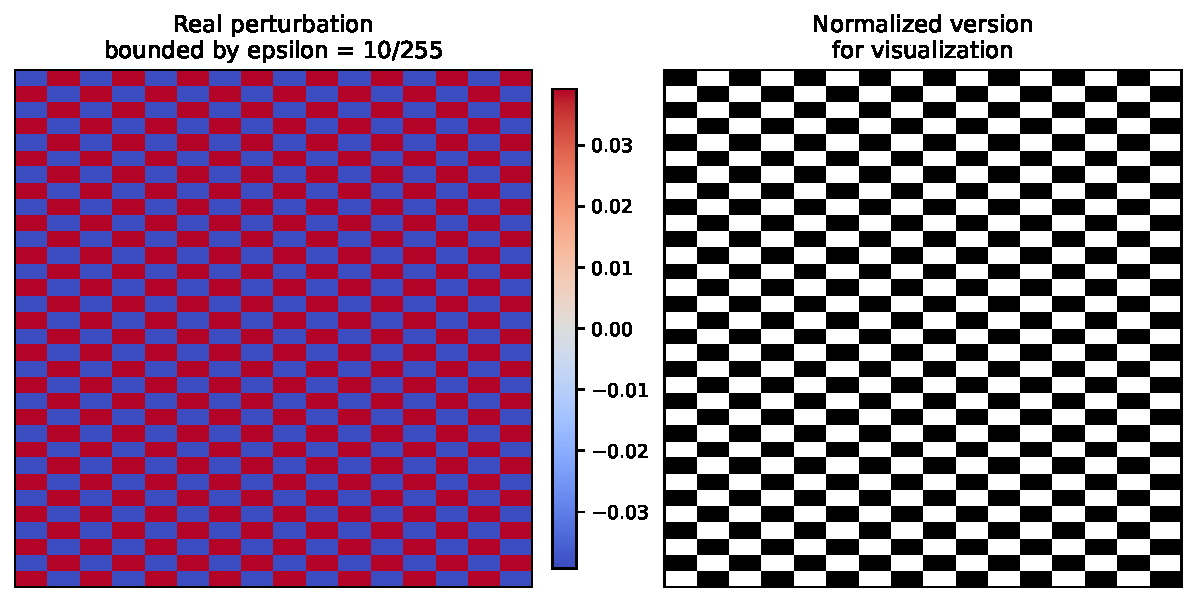
\includegraphics[width=0.55\textwidth]{figures/results/sfa_spatial_pattern_vgg_cifar10_en.pdf}
    \caption{Spatial pattern associated with the SFA perturbation at frequency $(16,24)$. The visualization is
    normalized to make the pattern's structure visible.}
    \label{fig:sfa_spatial_pattern_vgg_cifar10}
\end{figure}

\section{Measuring Frequency Sensitivity}
\label{sec:mesure_sensibilite_frequentielle}

Once the Fourier perturbations have been defined, their effect on the model must be measured.

\subsection{Definition of the Fool Ratio}
\label{subsec:def_fool_ratio}

Let $f$ be the model under study, and let $\mathcal{D}=\{x_1,\dots,x_M\}$ be a set of images. For a
given frequency $(u,v)$, let $\tilde{x}_k^{(u,v)}$ denote the image obtained by adding to $x_k$ the Fourier
perturbation associated with that frequency.

The \textit{fool ratio} measures the proportion of images for which the model's prediction changes
after perturbation:
\[
    \operatorname{FR}(u,v)
    =
    \frac{1}{M}
    \sum_{k=1}^{M}
    \mathbf{1}
    \left[
        f(x_k) \neq f\!\left(\tilde{x}_k^{(u,v)}\right)
    \right].
\]

This measure does not directly compare the prediction with the true label. It compares only the
model's prediction before and after perturbation. Thus, the attack counts as successful
on an image when the perturbation changes the model's decision.

The \textit{fool ratio} therefore indicates how effectively a frequency direction can change
predictions, regardless of the images' true class.

% \subsection{Stabilité entre heatmaps}

% Pour comparer les heatmaps obtenues avec différentes seeds d'entraînement, nous utilisons deux
% mesures de corrélation. Chaque heatmap est d'abord aplatie en un vecteur de taille $32\times32$,
% contenant les \textit{fool ratios} de toutes les fréquences.

% La corrélation de Pearson mesure si deux heatmaps ont une structure globale similaire en valeur. La
% corrélation de Spearman compare plutôt l'ordre relatif des fréquences, en remplaçant les valeurs par
% leurs rangs. Elle permet donc de vérifier si les fréquences les plus sensibles restent globalement les
% mêmes d'un entraînement à l'autre, même lorsque les valeurs exactes des \textit{fool ratios} changent
% légèrement.

\subsection{Generating Heatmaps}
\label{subsec:generation_heatmaps}

A frequency sensitivity heatmap is a matrix $H \in \mathbb{R}^{32\times32}$ in which each
entry corresponds to a frequency $(u,v)$. The value $H_{u,v}$ is the \textit{fool ratio} obtained when
the Fourier perturbation associated with that frequency is added to the test images.

The computation has three steps: first, we compute the model's predictions on clean images;
next, for each frequency, we apply the corresponding perturbation; finally, we measure
the proportion of predictions that change. This procedure is summarized in
Algorithm~\ref{algo:algorithme_heatmap}.

\begin{algorithm}[H]
\caption{Generating a frequency sensitivity heatmap}
\label{algo:algorithme_heatmap}
\begin{algorithmic}
\State \textbf{input}: model $f$, test images $\mathcal{D}$, amplitude $\epsilon$
\State \textbf{output}: heatmap $H \in \mathbb{R}^{32 \times 32}$
\State
\State $y \leftarrow f(\mathcal{D})$ \Comment{predictions on clean images}
\For{$u = 0$ \textbf{to} $31$}
    \For{$v = 0$ \textbf{to} $31$}
        \State $\delta_{u,v} \leftarrow$ construct the Fourier perturbation at frequency $(u,v)$
        \State $\tilde{\mathcal{D}}_{u,v} \leftarrow \operatorname{clip}_{[0,1]}(\mathcal{D} + \delta_{u,v})$
        \State $\tilde{y}_{u,v} \leftarrow f(\tilde{\mathcal{D}}_{u,v})$
        \State $H_{u,v} \leftarrow \operatorname{FoolRatio}(y,\tilde{y}_{u,v})$
    \EndFor
\EndFor
\end{algorithmic}
\end{algorithm}

\subsection{Selecting the Most Sensitive Frequency}
\label{subsec:choix_frequence_sensible}

Once the heatmap has been computed, we select the frequency that maximizes the \textit{fool ratio}:
\[
    (u^\star,v^\star)
    =
    \arg\max_{(u,v)}
    \operatorname{FR}(u,v).
\]

This frequency corresponds to the most effective Fourier perturbation among all those tested
in the protocol.

This selection is performed separately for CIFAR-10 and CIFAR-100. The resulting frequencies and
their interpretation are presented in Section~\ref{subsec:frequences_plus_sensibles}.

\section{Experimental Results}
\label{sec:resultats_experimentaux}

\subsection{Frequency Sensitivity Heatmaps}
\label{subsec:resultats_heatmaps}

The methodology described above allows us to construct frequency sensitivity maps
for the \texttt{VGGSmallBN} model. Figure~\ref{fig:heatmap_comparison_vgg_cifar10_cifar100}
compares the results obtained on our two datasets at the same perturbation amplitude,
set to $\epsilon = 10/255$.

\begin{figure}[H]
    \centering
    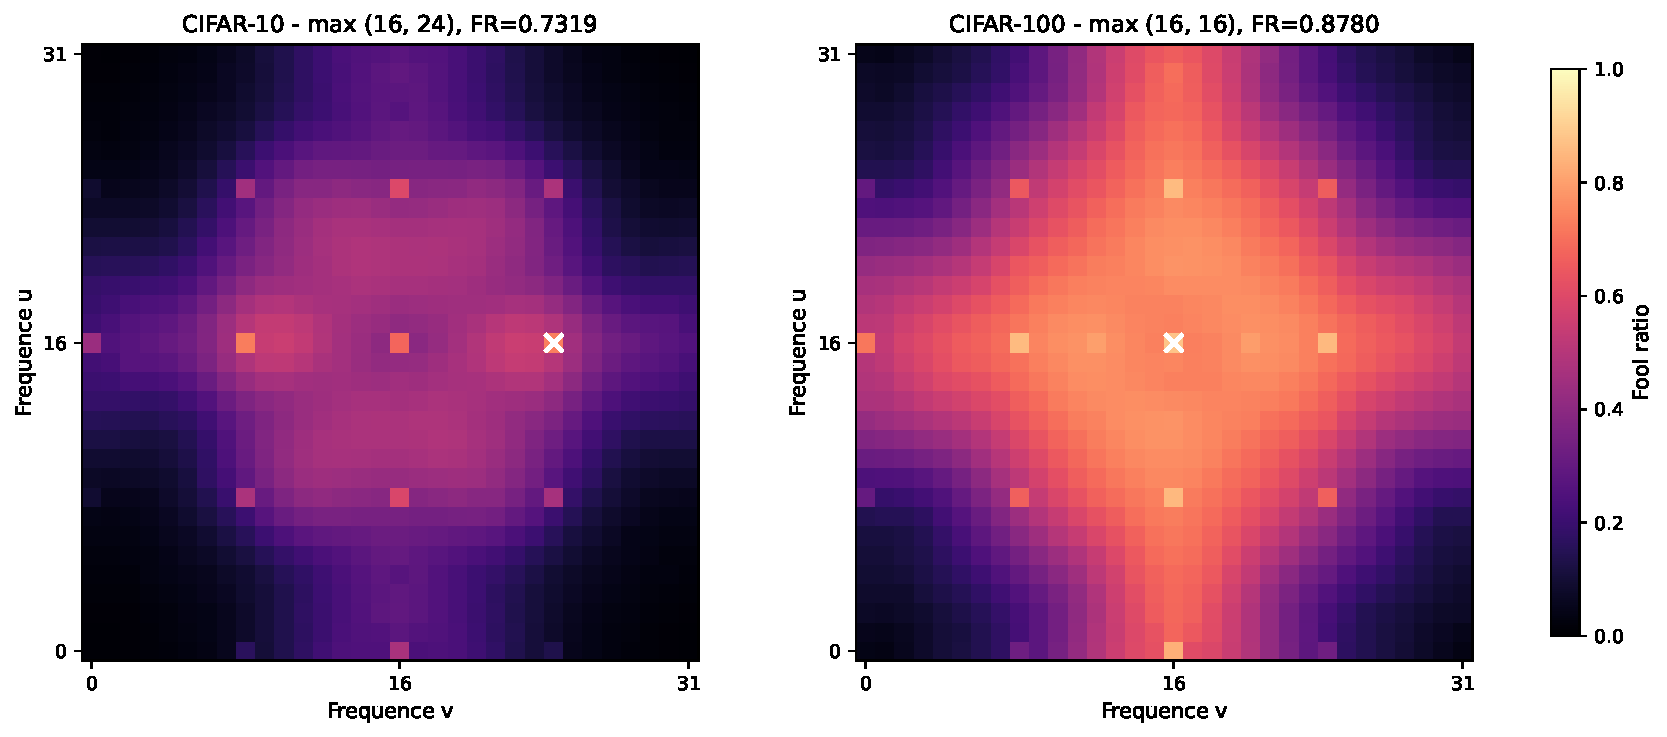
\includegraphics[width=0.7\textwidth]{figures/results/fourier_heatmap_comparison_vgg_cifar10_cifar100.pdf}
    \caption{Frequency sensitivity heatmaps for \texttt{VGGSmallBN} on CIFAR-10 and CIFAR-100.}
    \label{fig:heatmap_comparison_vgg_cifar10_cifar100}
\end{figure}
The main observation is that sensitivity is not uniform in the Fourier domain. Some
frequencies cause very few prediction changes, while others produce a
much higher \textit{fool ratio}.

Both heatmaps exhibit a structured organization, with regions of high sensitivity around
certain frequency lines and intersections, particularly near coordinates associated with $16$. This
structure suggests that the model's vulnerability is not a random effect, but depends on certain
preferred frequency directions.

A descriptive comparison with the mean spectrum of clean images appears in
Appendix~\ref{annexe:spectres_moyens_cifar}. This analysis aims to offer another way of interpreting
the results through the frequency statistics of the raw data.

To complement the heatmaps, Figure~\ref{fig:fool_ratio_histogram_comparison_vgg_cifar10_cifar100}
shows the distribution of \textit{fool ratios} over the $32 \times 32 = 1024$ frequencies tested.

On CIFAR-10, most frequencies have a weak or moderate effect, and only a few directions
achieve high \textit{fool ratios}. The model's sensitivity is therefore real, but relatively
localized in the frequency domain.

\begin{figure}[H]
    \centering
    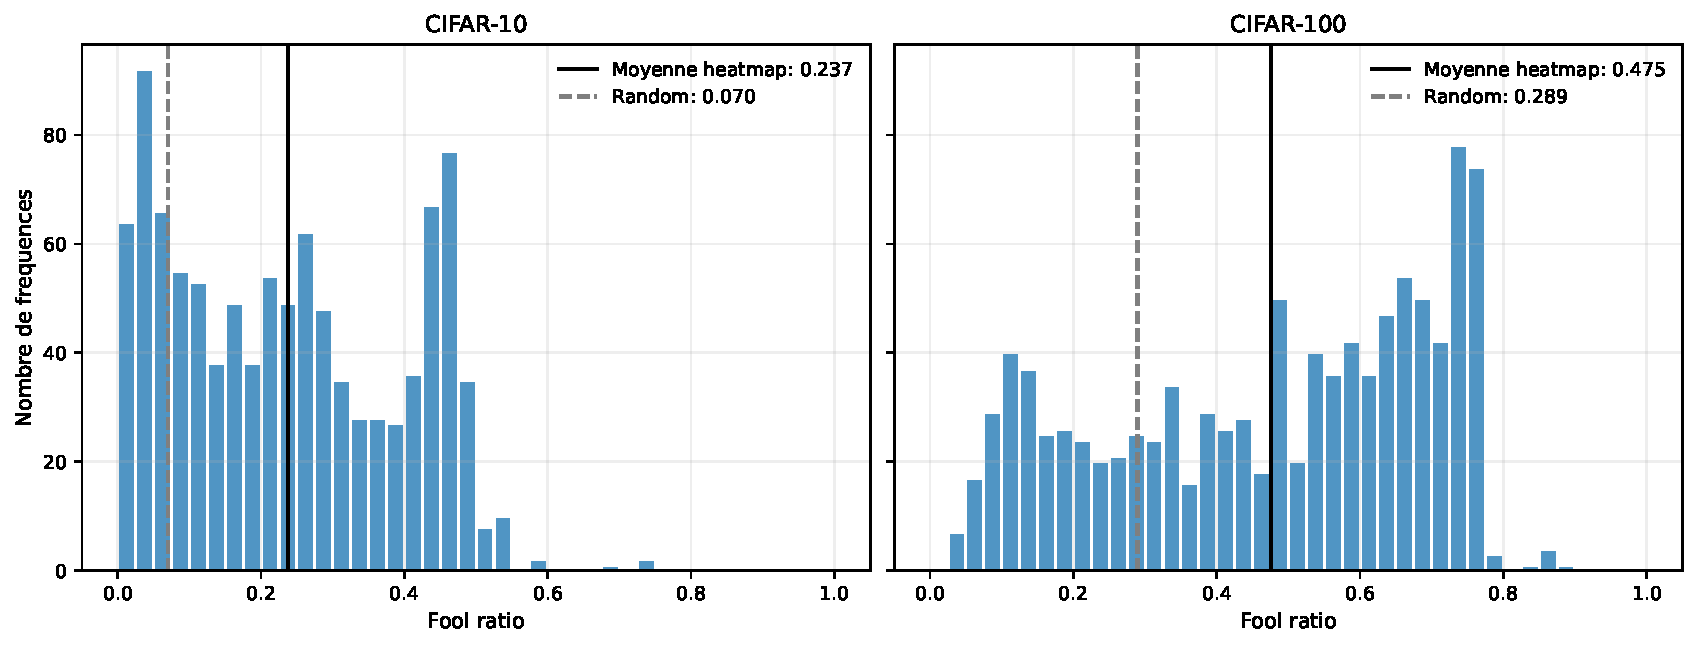
\includegraphics[width=0.9\textwidth]{figures/results/fourier_fool_ratio_histogram_comparison_vgg_cifar10_cifar100.pdf}
    \caption{Distribution of the \textit{fool ratios} obtained over all Fourier frequencies tested.}
    \label{fig:fool_ratio_histogram_comparison_vgg_cifar10_cifar100}
\end{figure}

On CIFAR-100, the distribution shifts to the right: the mean increases from $0.2375$ to $0.4755$.
The model is therefore more fragile overall, consistent with the greater difficulty of the
task discussed in Appendix~\ref{annexe:marges-logits}. However, this fragility remains structured: not all frequencies produce the same
effect, and some directions remain markedly more disruptive than others.

The histogram thus complements the visual interpretation of the heatmaps. It shows that sensitivity is
not only spatially nonuniform but also quantitatively highly dispersed. A small fraction
of the frequencies accounts for most of the disruptive effect.

\subsection{Most Sensitive Frequencies}
\label{subsec:frequences_plus_sensibles}

Analysis of the heatmaps identifies the most disruptive frequencies for each
dataset. Table~\ref{tab:frequences_plus_sensibles} presents the three frequencies with the
highest \textit{fool ratios}.

\begin{table}[H]
    \centering
    \begin{tabular}{c|cc|cc}
        & \multicolumn{2}{c|}{CIFAR-10} & \multicolumn{2}{c}{CIFAR-100} \\
        Rank & Frequency $(u,v)$ & \textit{Fool ratio} & Frequency $(u,v)$ & \textit{Fool ratio} \\
        \hline
        1 & $(16,24)$ & $0.7319$ & $(16,16)$ & $0.8780$ \\
        2 & $(16,8)$  & $0.7295$ & $(16,8)$  & $0.8585$ \\
        3 & $(16,16)$ & $0.6765$ & $(24,16)$ & $0.8565$ \\
    \end{tabular}
    \caption{Most sensitive frequencies for \texttt{VGGSmallBN} on CIFAR-10 and CIFAR-100.}
    \label{tab:frequences_plus_sensibles}
\end{table}

The dominant frequencies cluster around the same family of directions. On CIFAR-10, the top two frequencies,
$(16,24)$ and $(16,8)$, are conjugates modulo $32$ and, as expected, yield almost identical \textit{fool ratios}.


On CIFAR-100, the most sensitive frequency becomes $(16,16)$, which is its own conjugate modulo
$32$.

\subsection{Stability of Sensitive Regions Across Training Runs}
\label{subsec:stabilite_multi_seeds}

The preceding heatmaps show that some frequencies are much more sensitive than
others. However, an important question remains: is this structure specific to a
particular training run, or does it remain observable when the initialization seed
changes?

\begin{figure}[H]
    \centering
    \vspace{-10pt} 

    \begin{minipage}{0.35\textwidth}
        \centering
        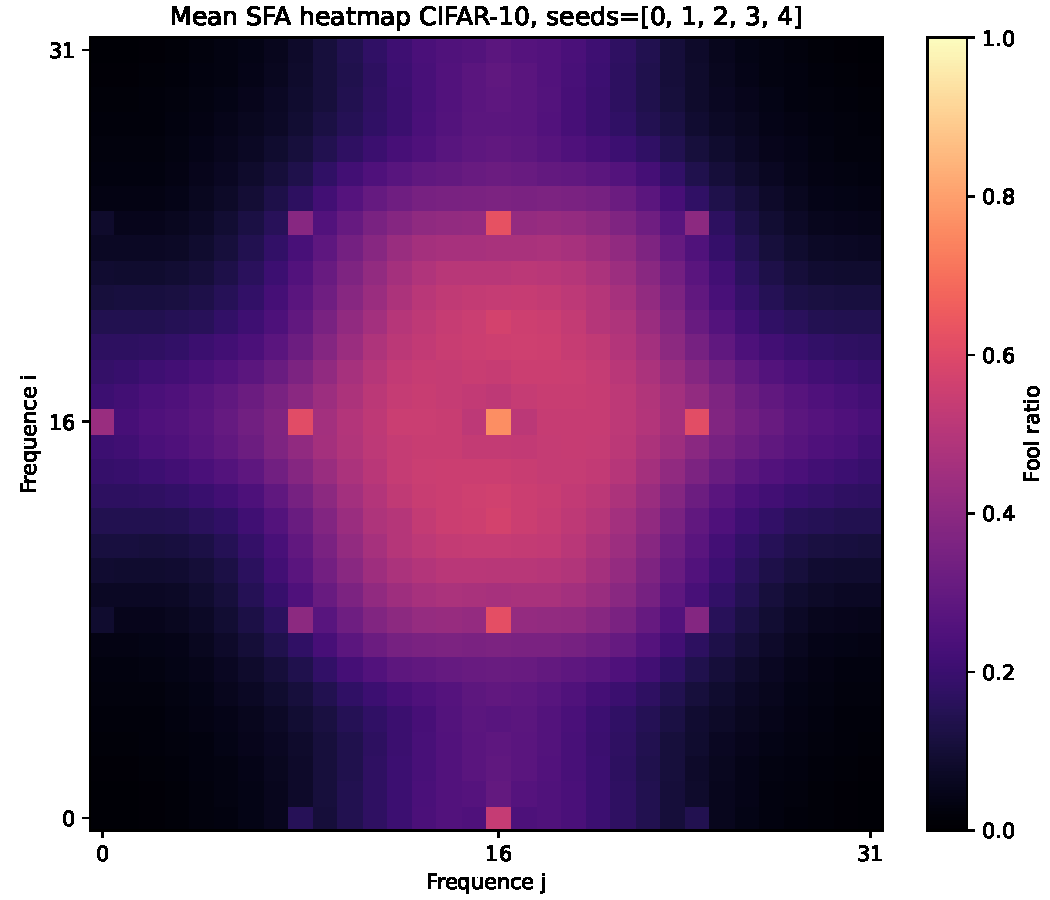
\includegraphics[width=\textwidth]{figures/results/stability_cifar10_heatmap_mean.pdf}
        \vspace{-5pt} 
        {\small (a) CIFAR-10 -- mean \textit{fool ratio}}
    \end{minipage}
    \hspace{0.05\textwidth} 
    \begin{minipage}{0.35\textwidth}
        \centering
        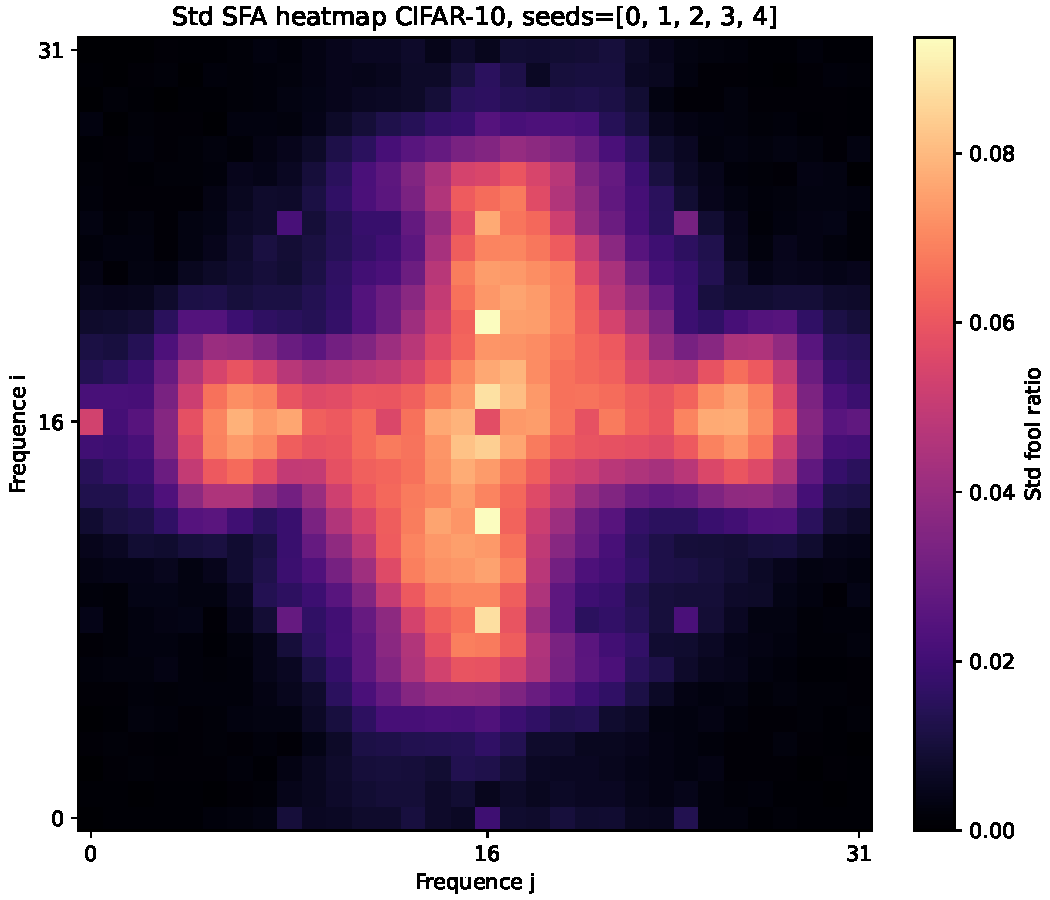
\includegraphics[width=\textwidth]{figures/results/stability_cifar10_heatmap_std.pdf}
        \vspace{-5pt}
        {\small (b) CIFAR-10 -- standard deviation}
    \end{minipage}

    \vspace{2pt} 

    \begin{minipage}{0.35\textwidth}
        \centering
        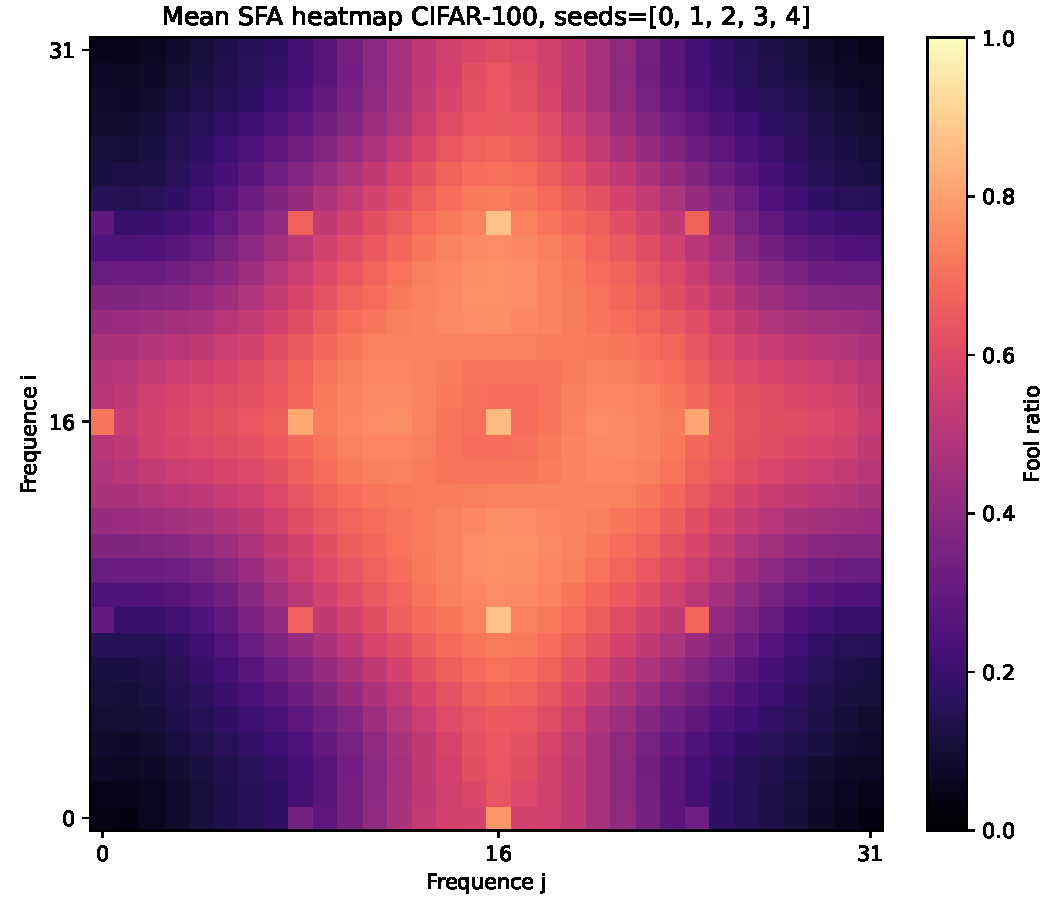
\includegraphics[width=\textwidth]{figures/results/stability_cifar100_heatmap_mean.pdf}
        \vspace{-5pt}
        {\small (c) CIFAR-100 -- mean \textit{fool ratio}}
    \end{minipage}
    \hspace{0.05\textwidth}
    \begin{minipage}{0.35\textwidth}
        \centering
        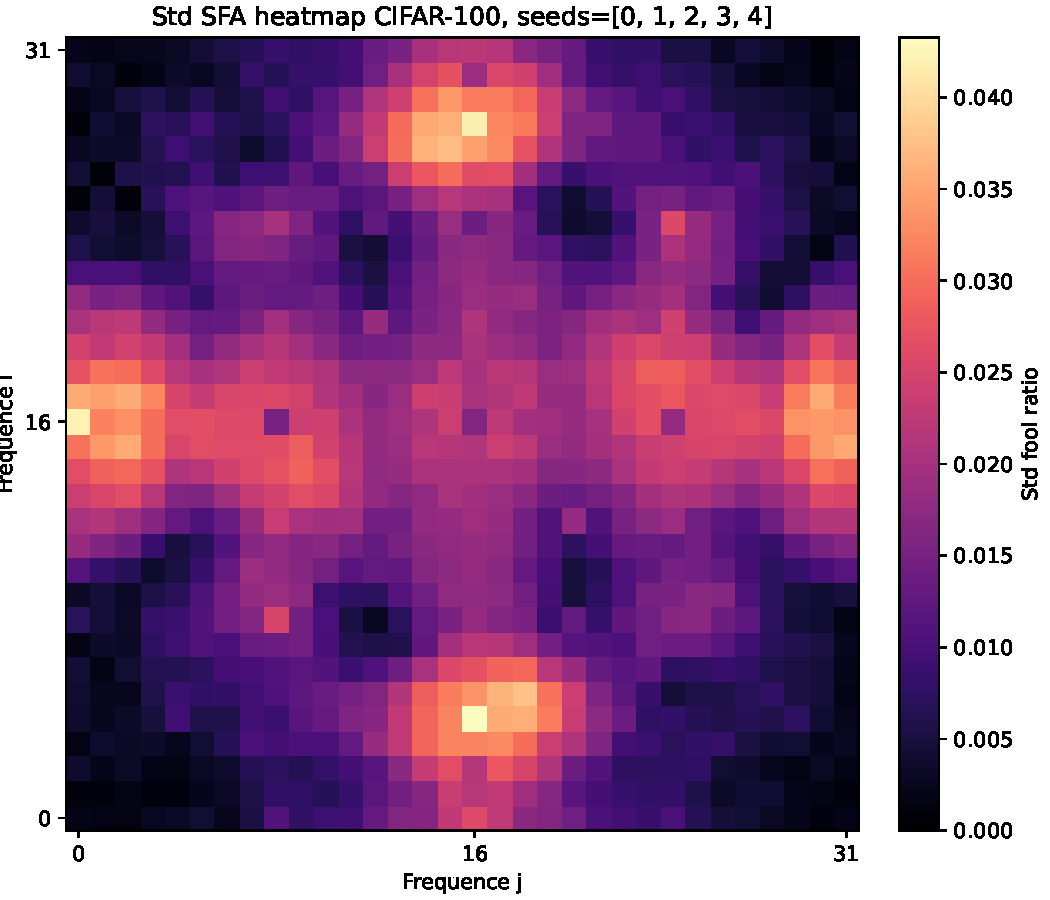
\includegraphics[width=\textwidth]{figures/results/stability_cifar100_heatmap_std.pdf}
        \vspace{-5pt}
        {\small (d) CIFAR-100 -- standard deviation}
    \end{minipage}

    \caption{Stability of the frequency sensitivity of \texttt{VGGSmallBN} on CIFAR-10 and CIFAR-100.}
    \label{fig:stability_cifar10_cifar100_mean_std}
\end{figure}

To answer this question, we repeated the experiment on CIFAR-10 and CIFAR-100 with five
independent training runs of \texttt{VGGSmallBN}. The training protocol remains identical
for each run. Only the seed changes.

For each dataset, Figure~\ref{fig:stability_cifar10_cifar100_mean_std} presents
the mean heatmap obtained across the five seeds and the standard deviation associated
with each frequency.

The results show that the overall heatmap structure remains highly stable across training runs.
On CIFAR-10, regions of high sensitivity remain localized around the same frequency regions,
particularly around the middle frequencies associated with the central axes. On CIFAR-100, this structure
is even more pronounced: a broad region of high sensitivity appears around the central frequencies.

% Cette stabilité est confirmée quantitativement par les corrélations entre heatmaps. Sur CIFAR-10, la
% corrélation de Pearson moyenne entre heatmaps est d'environ $0.976$, et la corrélation de Spearman
% moyenne d'environ $0.985$. Sur CIFAR-100, ces valeurs montent respectivement à environ $0.994$
% et $0.992$. Les heatmaps sont donc très proches d'un entraînement à l'autre, aussi bien en valeur
% qu'en classement relatif des fréquences.

Table~\ref{tab:stability_multiseed_metrics} summarizes the main metrics averaged across the five
seeds. Clean accuracy remains close to that of the main model, whereas accuracy after the attack
drops sharply. This shows that the high \textit{fool ratio} does correspond to an actual degradation
of model performance, rather than merely to prediction changes that have no effect on
correct classification.

\begin{table}[H]
    \centering
    \begin{tabular}{l|c|c}
        \hline
        Metric & CIFAR-10 & CIFAR-100 \\
        \hline
        Mean clean accuracy & $93.08\,\%$ & $72.50\,\%$ \\
        Mean best \textit{fool ratio} & $76.35\,\%$ & $87.64\,\%$ \\
        Mean accuracy after attack & $23.39\,\%$ & $11.83\,\%$ \\
        Success rate on initially correct images & $76.38\,\%$ & $85.18\,\%$ \\
        % Corrélation de Pearson moyenne entre heatmaps & $0.976$ & $0.994$ \\
        % Corrélation de Spearman moyenne entre heatmaps & $0.985$ & $0.992$ \\
        \hline
    \end{tabular}
    \caption{Summary of the stability experiment across multiple seeds on CIFAR-10 and CIFAR-100.}
    \label{tab:stability_multiseed_metrics}
\end{table}

\subsection{Internal Amplification of Sensitive Frequencies}
\label{subsec:amplification_interne_sfa}

The preceding heatmaps show that some Fourier frequencies produce markedly higher \textit{fool ratios}
than others. To better understand this phenomenon, we analyzed how
these perturbations propagate inside the network.

For a perturbation \(\delta\), let \(G_l(\delta)\) denote the normalized amplification measured at
layer \(l\). This quantity compares the mean norm of the activation change caused by the
perturbation with the norm of the input perturbation. It therefore allows us to compare the relative effect of
different frequencies within the network's internal blocks and at the logit level.

To make this analysis more robust, we repeated it on the five checkpoints used in
the stability experiment across multiple seeds. Frequencies are grouped using the mean heatmap:
the \(50\) most sensitive frequencies, \(50\) frequencies of intermediate sensitivity, and the \(50\)
least sensitive frequencies. The primary frequency is the best frequency on average
across the five seeds.

\begin{figure}[H]
    \centering
    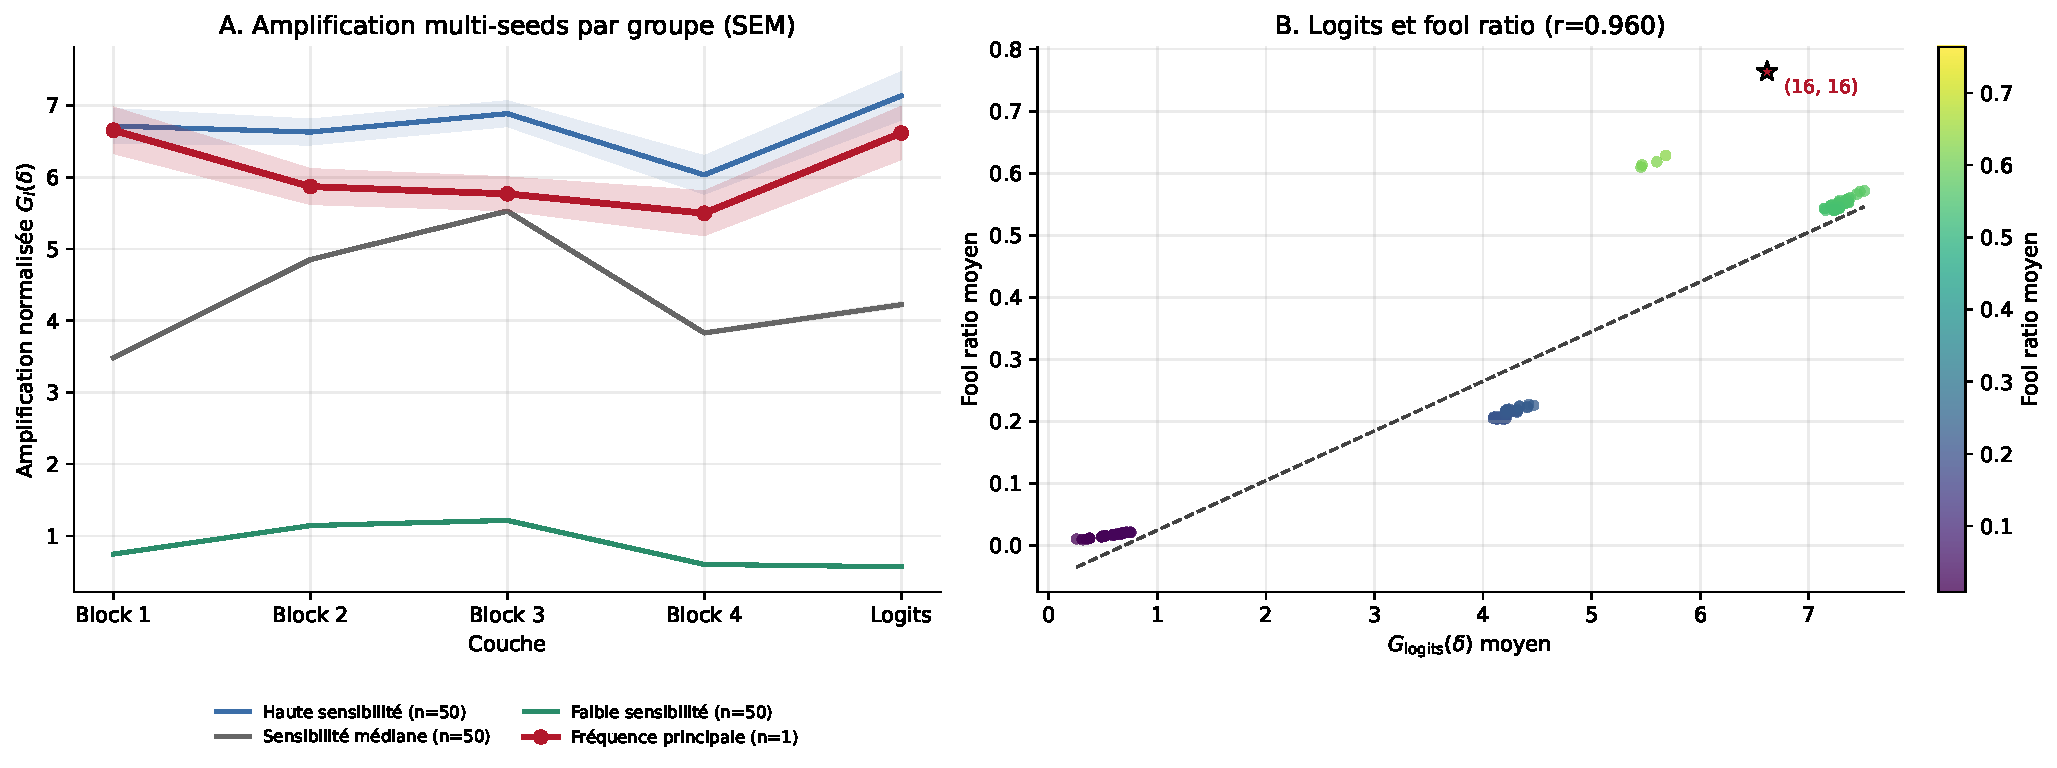
\includegraphics[width=\textwidth]{figures/results/layerwise_frequency_sensitivity_analysis_vgg_cifar10_multiseed.pdf}
    \caption{Analysis of the internal amplification of Fourier perturbations across multiple seeds in
    \texttt{VGGSmallBN} on CIFAR-10. Left: frequencies are grouped by their
    mean \textit{fool ratio}. Bands indicate the standard error across the five seeds. Right:
    mean amplification at the logit level is compared with the mean \textit{fool ratio}.}
    \label{fig:layerwise_frequency_sensitivity_multiseed}
\end{figure}

Figure~\ref{fig:layerwise_frequency_sensitivity_multiseed} shows that, as expected, the most
sensitive frequencies also produce the greatest internal amplification.

The right panel shows a strong correlation between mean amplification at the logit level
and the mean \textit{fool ratio}. This suggests that the model's final sensitivity is related not only
to the chosen pair $(u, v)$, but also to how this perturbation is propagated and
amplified by the network.

This observation connects with the theoretical framework and the local interpretation introduced in the
previous chapter: although the real network is not globally linear, certain
frequency directions seem to be amplified more by its local behavior, which may explain
their greater effect on predictions.

A more detailed visualization of the internal heatmaps by layer is provided in Appendix~\ref{annexe:heatmaps_internes_couches}.

\subsection{Comparison with Random Noise}
\label{subsec:comparaison_bruit_aleatoire}

To verify that the high values obtained by SFA are not solely due to the perturbation's
amplitude, we compare the best Fourier direction with a random-noise
baseline. In this baseline, each pixel is perturbed independently by uniform noise
bounded within the same amplitude interval. The constraint is therefore the same as for SFA:
\[
    \|\delta\|_{\infty} \leq \epsilon,
    \qquad
    \epsilon = 10/255.
\]
The difference lies in the perturbation's structure: SFA uses a coherent frequency pattern,
whereas the random baseline does not favor any particular direction.

\textbf{TO DO: }
We should ensure that $\|\delta_{SFA}\|_{2} = \|\delta_{random}\|_{2}$

For each dataset, Figure~\ref{fig:sfa_vs_random_comparison_vgg_cifar10_cifar100} compares
the \textit{fool ratio} of the best SFA frequency with the mean \textit{fool ratio} obtained using random
noise.

\begin{figure}[H]
    \centering
    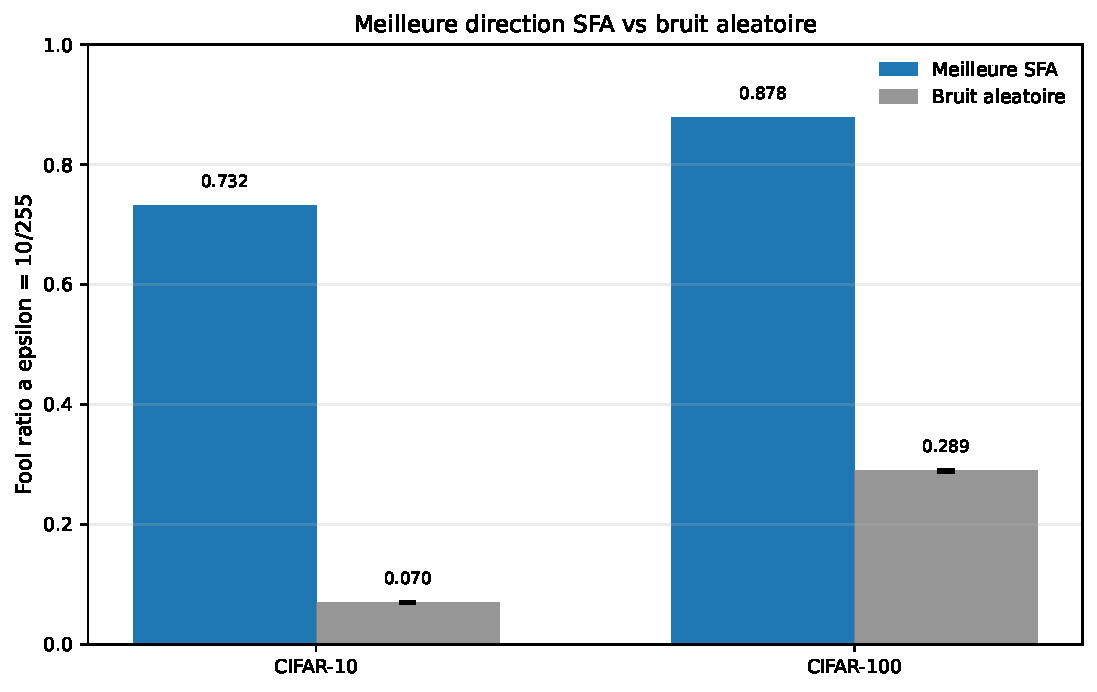
\includegraphics[width=0.85\textwidth]{figures/results/sfa_vs_random_comparison_vgg_cifar10_cifar100.pdf}
    \caption{Comparison between the best SFA direction and uniform random noise of the same amplitude
    $\epsilon = 10/255$. For random noise, the error bar represents the standard deviation over 100 trials.}
    \label{fig:sfa_vs_random_comparison_vgg_cifar10_cifar100}
\end{figure}

On CIFAR-10, the difference is striking: the best Fourier direction achieves a
\textit{fool ratio} of $0.7319$, whereas the mean for random noise is only $0.0704$.
The Fourier perturbation is therefore approximately ten times as effective as random noise of the same
amplitude. This result indicates that the observed vulnerability cannot be explained solely by
the size of the perturbation.

On CIFAR-100, random noise is already more disruptive, with a mean \textit{fool ratio} of
$0.2892$, confirming that the model trained on CIFAR-100 is more fragile overall. However,
the best SFA direction reaches $0.8780$, approximately three times the mean level for random noise.

\subsection{Effect of Perturbation Amplitude}
\label{subsec:effet_amplitude_epsilon}

So far, the main results have been obtained with $\epsilon = 10/255$. This value allows us to
compare our results with the original protocol, but it can produce visible patterns in
very low-resolution images. However, an adversarial attack aims to remain
barely perceptible to humans. We therefore test whether the most sensitive frequencies retain an effect at
lower values of $\epsilon$.

To do so, we fix the most sensitive frequency for each dataset and then vary
$\epsilon$ over the following set:
\[
    \epsilon \in
    \left\{
        \frac{1}{255},
        \frac{2}{255},
        \frac{3}{255},
        \frac{5}{255},
        \frac{10}{255}
    \right\}.
\]

\begin{figure}[H]
    \centering
    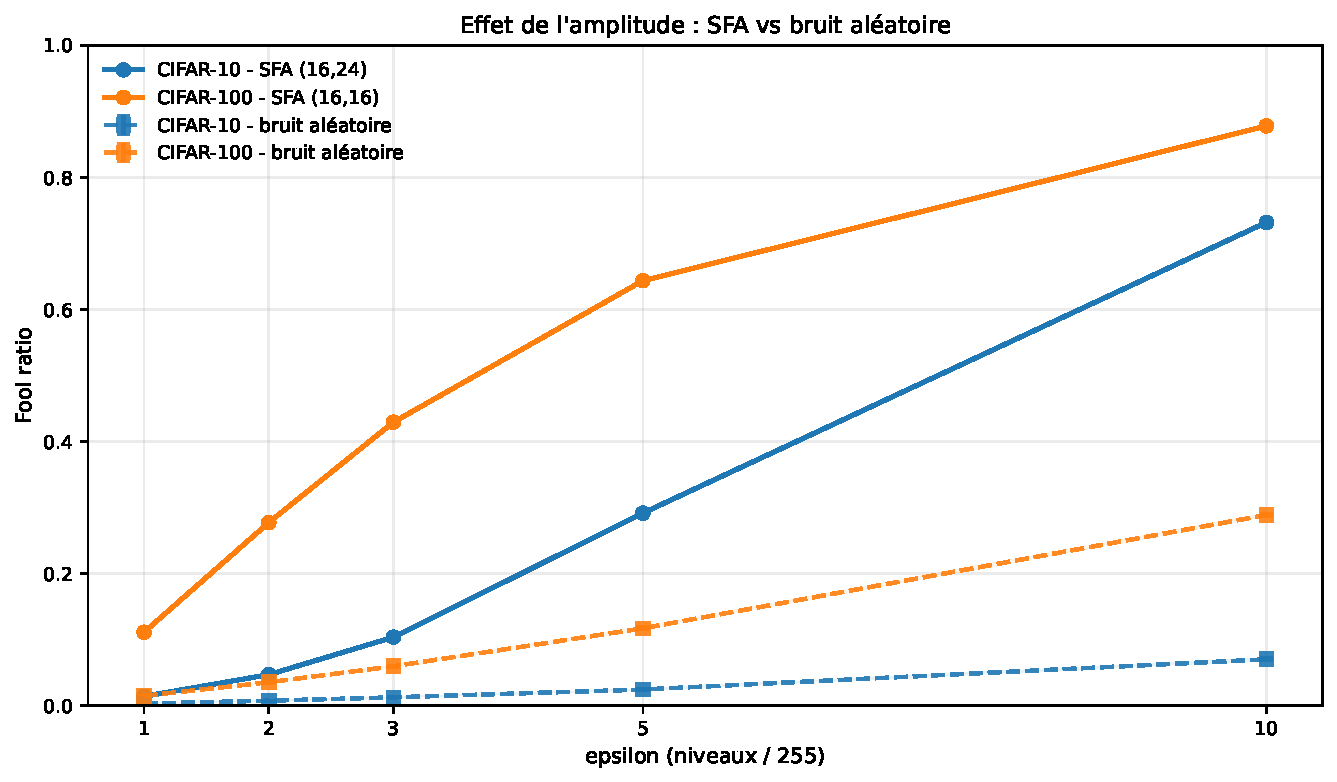
\includegraphics[width=0.55\textwidth]{figures/results/sfa_epsilon_sweep_with_random_comparison_vgg_cifar10_cifar100.pdf}
    \caption{\textit{Fool ratio} as a function of amplitude $\epsilon$ for the best SFA frequency
    on each dataset.}
    \label{fig:sfa_epsilon_sweep_comparison_vgg_cifar10_cifar100}
\end{figure}

Figure~\ref{fig:sfa_epsilon_sweep_comparison_vgg_cifar10_cifar100} shows a steady
increase in the \textit{fool ratio} as $\epsilon$ increases. This behavior is expected: the larger the
perturbation, the more it changes the input image and the more likely it is to alter the
model's prediction. However, it also confirms that, in this setting, perturbation amplitude
is an important factor in attack effectiveness, requiring a less subtle perturbation
to obtain a more substantial effect.

\begin{figure}[H]
    \centering
    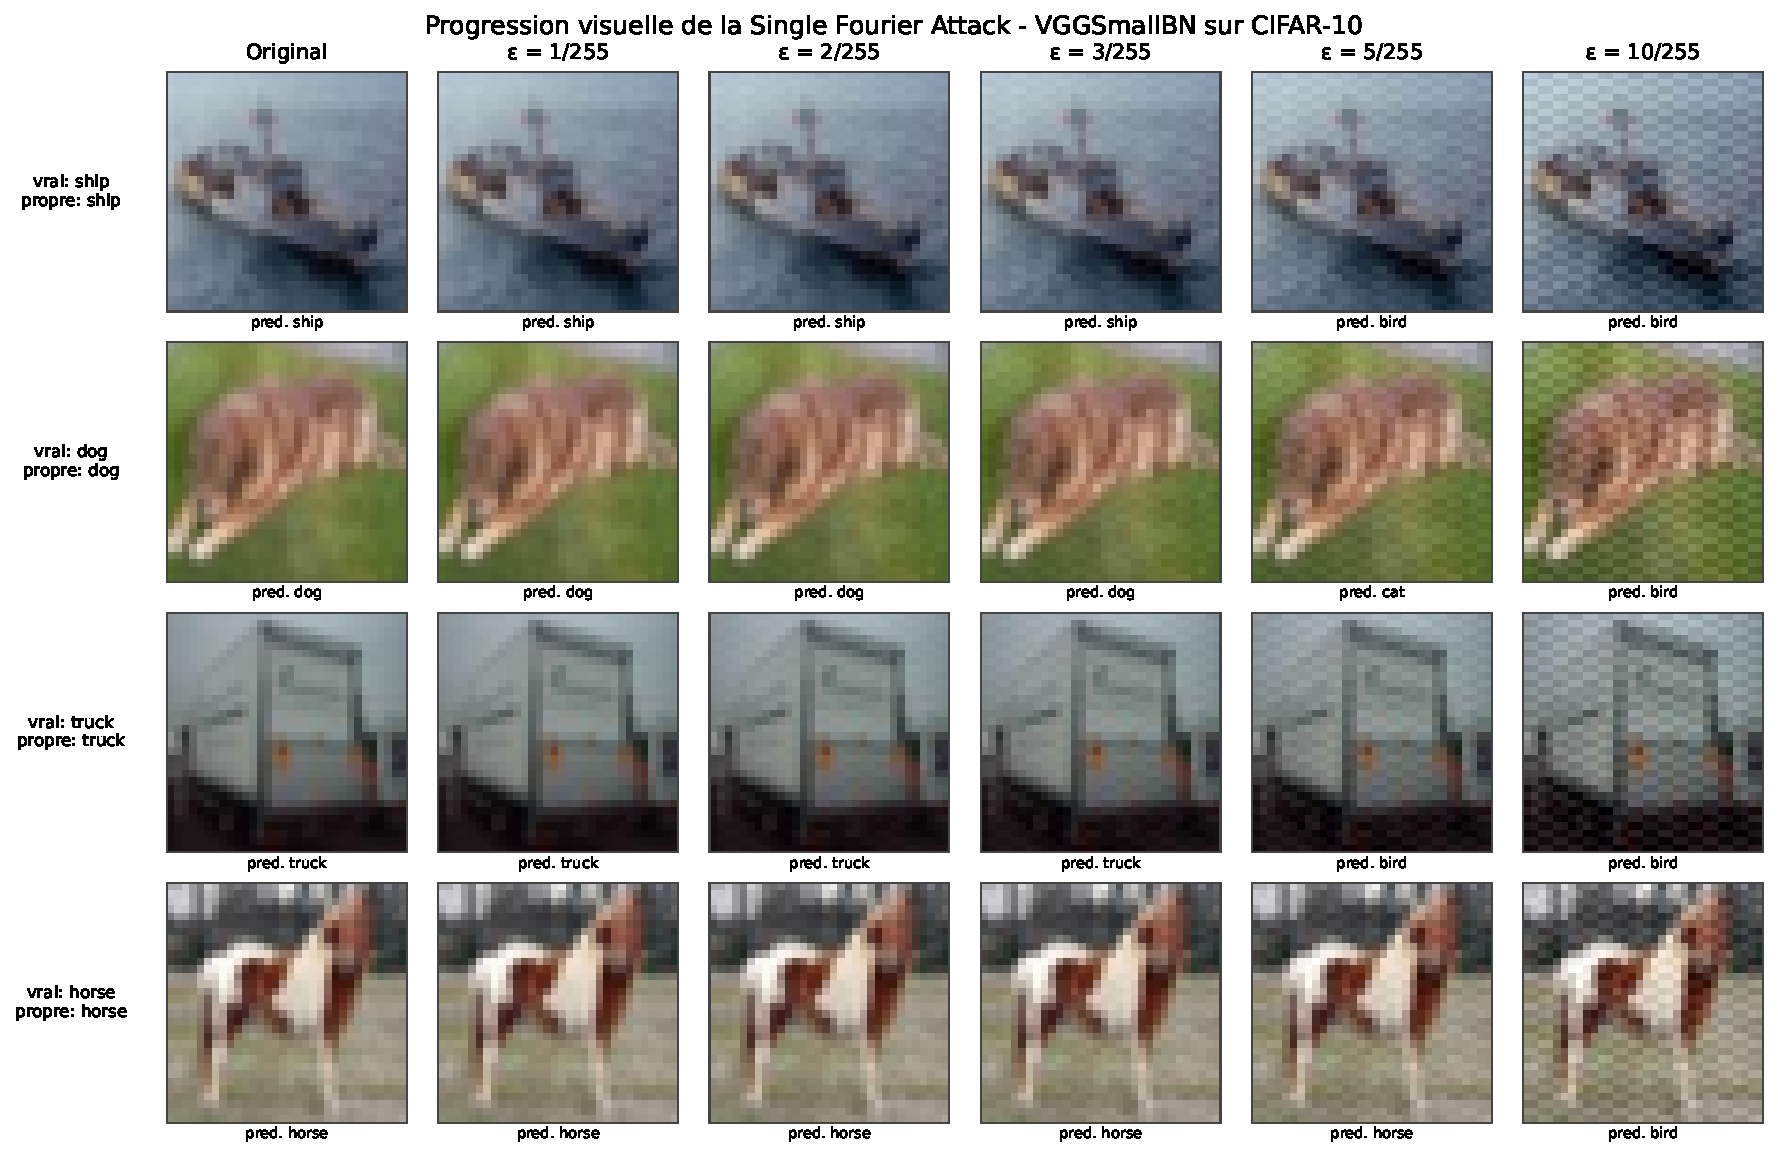
\includegraphics[width=1\textwidth]{figures/results/sfa_visual_progression_vgg_cifar10.pdf}
    \caption{Visual progression of a \textit{Single Fourier Attack} on CIFAR-10 images.}
    \label{fig:sfa_visual_progression_vgg_cifar10}
\end{figure}

As Figure~\ref{fig:sfa_visual_progression_vgg_cifar10} illustrates, increasing the amplitude makes the
Fourier pattern increasingly intrusive. In particular, from $\epsilon = 3/255$ onward, the
structured grid-like perturbation begins to become clearly visible to the naked eye.

These observations should nevertheless be qualified. The experiments use
very low-resolution images ($32\times32$ pixels) and a deliberately limited architecture
(\texttt{VGGSmallBN}). The conclusions should therefore not be generalized directly to
high-resolution images or much deeper architectures. They do, however, show that,
in our experimental setting, the effect of Fourier perturbations depends strongly on amplitude.

\subsection{Connection with the Theoretical Framework}
\label{subsec:discussion_lien_cadre_theorique}

The experimental results in this chapter allow us to revisit the theoretical framework
developed in the previous chapter. In the idealized linear model, Fourier functions emerge
as preferred directions of convolution operators. In a real CNN, this property
no longer applies directly to the entire network, but it may remain locally relevant through
the model's Jacobian.

The experimental heatmaps support this interpretation. If all frequency directions
were equivalent for the model, the sensitivity maps would be much more uniform. Yet this
is not what we observe: some frequencies produce markedly higher \textit{fool ratios}
than others, even though all perturbations satisfy the same $\ell_\infty$ constraint.

Stability across multiple seeds reinforces this interpretation. The sensitive regions do not seem to depend
solely on a particular network initialization: they remain visible when training is
repeated with different seeds. The comparison with random noise also shows that the effect
arises not only from the perturbation's amplitude, but also from its frequency structure.

These results show that the intuition derived from the theoretical framework remains
experimentally observable for \texttt{VGGSmallBN}: some Fourier directions are more disruptive than others,
consistent with local amplification of these directions within the network.

\paragraph{Influence of channel mixing.}

Previously, we considered the possibility that a sensitive direction may also involve mixing
the color channels, in the form $a \otimes \varphi_{u,v}$. The main protocol uses a simplified version of
this idea: the same Fourier pattern is applied to all three channels, corresponding to a
color direction of the form $(1,1,1)$.

A supplementary analysis of this simplification is provided in Appendix~\ref{annexe:color_sfa}.
It aims to show that the choice of channel mixing has a negligible effect compared with selecting the direction that maximizes attack amplification.

\section{Chapter Summary}
\label{sec:synthese_chapitre4}

The experiments confirm that the sensitivity of \texttt{VGGSmallBN} to Fourier
perturbations is highly nonuniform. On both CIFAR-10 and CIFAR-100, some frequencies
cause far more prediction changes than others, even though all perturbations
satisfy the same $\ell_\infty$ constraint.

This structure remains stable across several independent training runs and substantially exceeds the effect
of random noise of the same amplitude. However, the $\epsilon$ sweep shows that
attack effectiveness depends strongly on amplitude, particularly for low-resolution
images such as those in CIFAR.

Finally, the internal analysis suggests that the most sensitive frequencies are also those amplified
most strongly in the network's representations. These observations do not prove that the real model
behaves as a global linear operator, but they show that the frequency structure
identified in the theoretical setting remains partly visible in the model's local behavior.
